\section{Gestione dinamica peer/superpeer}
La necessità di rendere dinamica l'interazione che esiste tra un supernodo e i suoi nodi associati nasce dal fatto che, in un 'architettura P2P del tipo parzialamente ditribuita (ovvero ibrida), il sistema complessivo è progettato per trarre vantaggio dalla potenza di calcolo e di memorizzazione di un'ampia rete di calcolatori. E' di fondamentale importanza che sia garantita la capacità della struttura di trattare l'instabilità e la connettività in modo variabile e a seconda della situazione della rete di connessione, con la conseguenza di essere auto-adattabile e tollerante ai guasti.
In generale, i requisiti base che il sistema deve rispettare per la selezione dei SuperPeer sono:

\begin{itemize}
\item presenza di una quantità di superpeer proporzionale al numero totale di nodi;
\item numero massimo di peer connessi limitato per ogni superpeer;
\item selezione di peer  che possono diventare superpeer in base alle caratteristiche tecniche che hanno. Non tutti i peer infatti possiedono le capacità necessarie a svolgere il ruolo di supernodo, per questo motivo la rete è periodicamente aggiornata (utilizzando il valore di RATING) al fine di garantire le migliori prestazioni offerte dal sistema;
\end{itemize}

\subsection{Connessione ad un superpeer}
Le specifiche descritte sopra, servono innanzitutto per gestire il fatto che potenzialmente potrebbero esserci dei guasti o degli errori nella rete che causerebbero il crollo dei superpeer. In questo caso, dopo l'evento di timeout in cui il superpeer dimostra di non essere piu attivo, tutti i suoi peer associati rimarrebbero esclusi dal sistema e avranno bisogno di effettuare una nuova connessione.Il peer chiama quidni la funzione change\_SP, con la quale, utilizzando un ulteriore funzione detta connect\_to\_SP, il peer può cambiare il suo superpeer tramite una nuova join al server e in seguito con la creazione di una nuova connessione con il superpeer che gli è piu vicino (potrebbe verificarsi che il peer nel frattempo venga eletto a sua volta supernodo e che esegua il codice relativo).\linebreak

\subsection{Elezione di un nuovo superpeer}
Un'altra situazione problematica potrebbe essere quella in cui il peer che vuole accedere alla rete non trovi un superpeer disponibile, poichè tutti hanno già raggiunto il limite massimo di connessioni disponibili da accettare (o anche perchè la join\_UDP non è andata a buon fine dopo tutti i tentativi disponibili). Serve perciò un nuovo superpeer che accetti nuove connessioni, e questo messaggio viene inviato dal peer ad un superpeer, preso dalla lista di indirizzi restituiti dal server dopo la join.\linebreak
Il messaggio viene inviato utilizzando la funzione eleggi\_UDP: tale procedura informerà il superpeer più vicino ( comando di eleggi\_UDP() ) della necessità di un nuovo superpeer; il peer quindi invierà un messaggio strutturato di “elez” al superpeer, il quale proverà ad eleggere il suo best peer a superpeer in modo tale da far connettere il peer al nuovo superpeer ( che è perciò anche il miglior nodo presente nella sottorete in quel momento a livello di rating).
Il superpeer invierà al best peer un messaggio di tipo "nwsp" e il peer che riceverà questo messaggio abbandonerà il superpeer corrente, diventando a sua volta superpeer, e farà la join a se stesso. Se non ci sono problemi nell'avvio del processo di superpeer, il best peer invierà al suo superpeer precedente un messaggio di "ackE" per indicare che l'elezione è andata a buon fine.\linebreak
Il superpeer che riceve ackE invierà un messaggio di "crsp" al peer indicando l'ip del nuovo superpeer (se l'elezione è andata bene). A questo punto, dopo aver ricevuto la conferma tramite un messaggio di "crsp" (crea sp), il peer esegue una nuova join all'indirizzo ricevuto, e la funzione restituirà 1 se la connessione verrà accettata e stabilita tra peer e nuovo superpeer.\linebreak

\begin{figure}[h]
\centering
{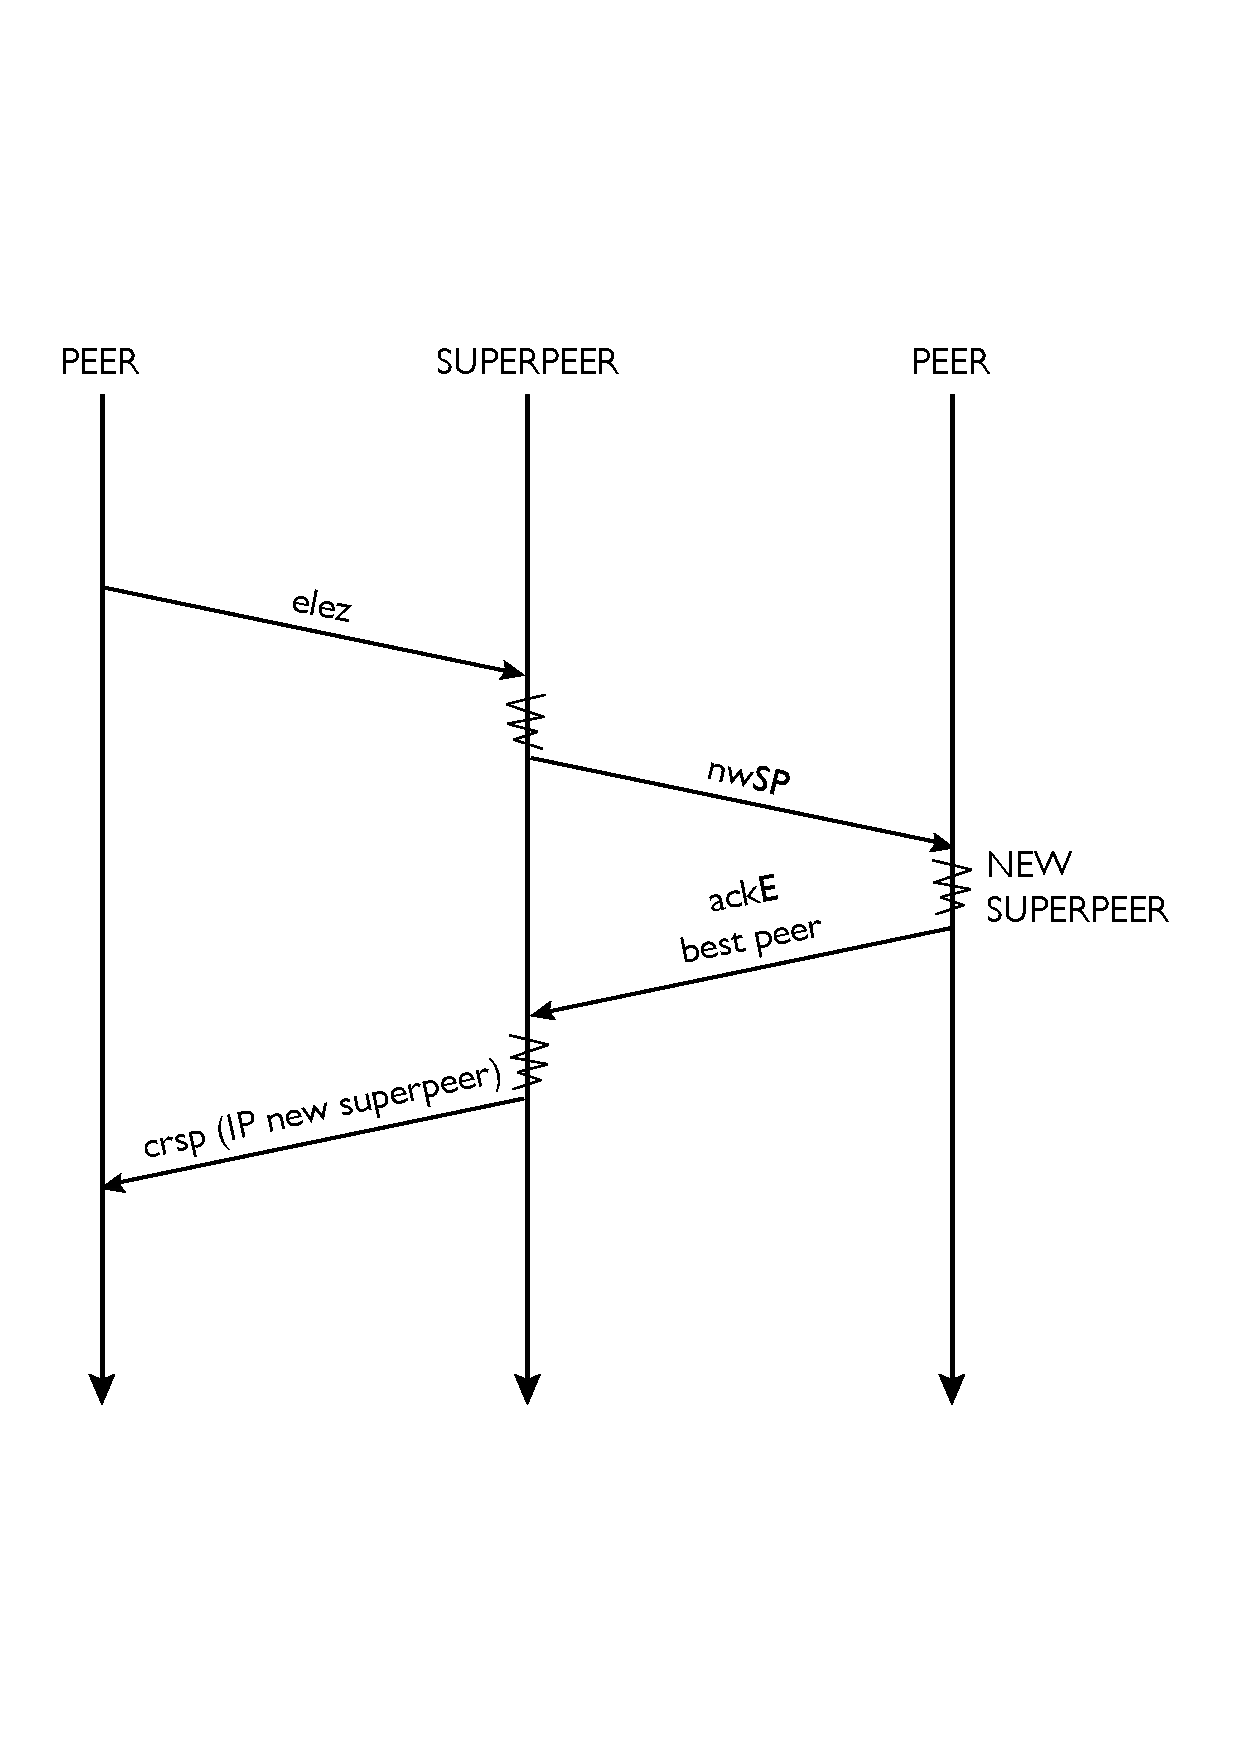
\includegraphics[width=8cm]{img/eleggi}}
\caption{elezione di un peer a superpeer\label{elezione}}
\end{figure}

\subsection{Leave del superpeer}
L'operazione di leave consiste nell'uscita di un superpeer dal sistema. A differenza dell'uscita di un semplice peer, in cui è sufficiente che il supernodo cancelli l'indirizzo ip e il filtro di bloom associato, la leave del superpeer deve gestire piu aspetti. Per prima cosa il superpeer informa il server di bootstrap, il quale cancella le informazioni relative al supernodo da cui ha ricevuto il messaggio (indirizzo IP piu filtro dei file condivisi dal lato peer); successivamente cerca e registra l'indirizzo del suo best peer ( il miglior nodo a livello di rating tra tutti gli altri connessi) e gli invia un messaggio di "nwsp" (anche nella fase di elezione veniva mandato lo stesso messaggio, ma a quest'ultimo ora viene impostato ad 1 un flag che segnala che il nuovo superpeer prenderà il posto di quello vecchio, anzichè diventarne uno nuovo per accettare nuove connessioni); infine ogni peer viene avvisato del cambio del supernodo, ricevendo un messaggio di leave e contemporaneamente l'indirizzo IP del best peer che nel frattempo è diventato il nuovo superpeer e a cui potranno connettersi. Il processo del superpeer che ha effettuato la leave termina, mentre il processo peer associato proseguirà instaurando la connessione a lnuovo indirizzo ricevuto.
Per come è stata strutturata l'architettura del sistema, il comando leave potrebbe essere effettuato da un peer che allo stesso tempo è attivo anche come superpeer. In questo caso le operazioni rimangono le stesse per entrambi: il peer invia una leave al superpeer (cioè a sè stesso), il superperr riconosce il suo indirizzo, cancella le informazioni associate al nodo che ha inviato il comando e allo stesso tempo effettua la leave nello stesso modo in cui è stata descritta sopra, facendo terminare di fatto sia il processo peer che quello superpeer.

\subsection{Switch tra peer e superpeer}
Svolge un ruolo importante anche l'aggiornamento periodico del rating all'interno sia della sottorete tra peer e superpeer sia della rete di overlay tra i vari superpeer. In questo modo infatti è possibile garantire buone prestazioni del sistema eleggendo al ruolo di supernodo ( che dal punto di vista dell'utilizzo delle risorse è il piu impegantivo) i nodi migliori che entrano man mano nel sistema. \linebreak
Ogni volta che un peer "pinga" il suo superpeer (ed anche quando viene effettuata un operazione di update dei file condivisi), invia a quello anche il suo rating aggiornato, e nel caso in cui si colleghi un nuovo peer che abbia rating maggiore (il doppio) rispetto al supernodo a cui si è collegato, viene attivata una fase di switch tra il superpeer e il miglior peer.\linebreak
Tale fase consiste di poche fasi:
\begin{itemize}
\item Leave al bootstrap del superpeer
\item Invio messaggio di elezione al peer designato con flag di switch
\item Leave forzata dei peer connessi al superpeer
\end{itemize}

\begin{figure}[h]
\centering
{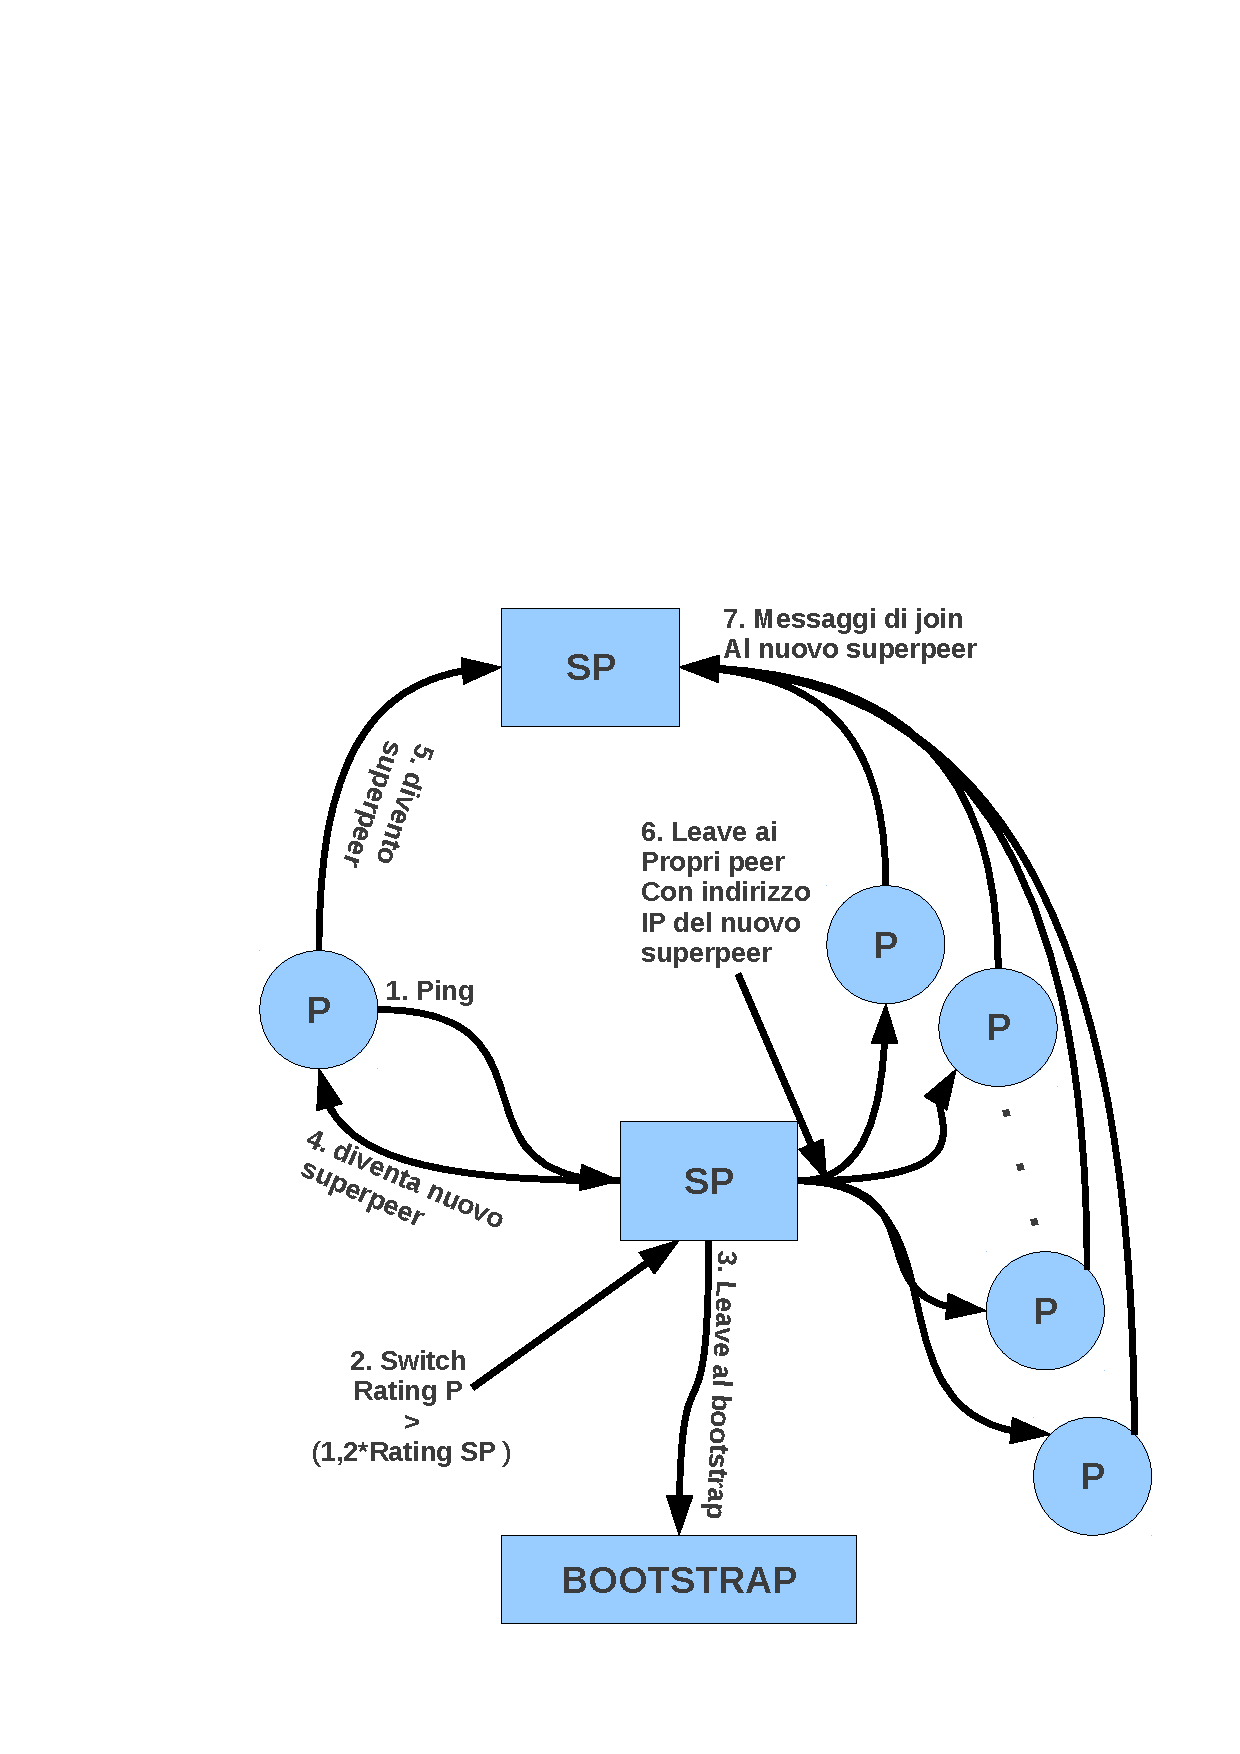
\includegraphics[width=7cm]{img/Switch}}
\caption{Switch del superpeer con un suo peer con rating migliore almeno del 20 \% \label{switch}}
\end{figure}

Il nuovo peer diventa superpeer e la rete viene aggiornata di questo scambio, sia con la register al server, sia con gli altri peer che dovranno collegarsi al nuovo superpeer ed infine con l'instaurazione di nuove connessioni TCP con gli altri supernodi della rete di overlay.\linebreak
Il flag di switch identifica un pacchetto di tipo "nwsp" con campo dati impostato a "s" al contrario del messaggio di nuovo superpeer usato nell'elezione semplice che ha campo dati vuoto. Tale flag permette di bloccare l'inoltro del messaggio "crsp" il quale senza flag sarebbe stato inviato al peer che ha generato la procedura di switch e questo sarebbe inutile.\linebreak
Da notare come il valore del rating non dipenda solo dalle capacità tecniche di un nodo, ma anche dal suo tempo di permanenza in rete; viene così garantita una stabilità maggiore all'applicazione, che potrà fare affidamento su calcolatori potenti e allo stesso tempo affidabili per quanto riguarda la continuità del funzionamento.\linebreak

\subsection{Unione di due superpeer}
Anche i superpeer scambiano tra di loro messaggi di aggiornamento rating, ma per un motivo diverso: se nella rete di overlay coesistono ad esempio due superpeer con tasso di occupazione minore del 20\% (dove per tasso di occupazione si intende il numero di peer connessi al superpeer rispetto al numero totale che in realtà potrebbero essere collegati contemporaneamente), avviene una fusione tra i due. Quando uno di loro riceve una leave da un suo peer, viene controllata la lista dei nodi che gli sono ancora connessi; se il numero è abbastanza piccolo (minore di 20), il superpeer chiama la funzione getSuperPeerBassaOccupazione(), ottenendo il numero di supernodi che come lui hanno un'occupazione minore del 20\%. Se ne esiste almeno uno in questa situazione, invia un comando di merge (fusione appunto) con allegato il valore del suo rating: nel caso in cui il superpeer che manda il messaggio ha rating maggiore, l'altro risponde con un messaggio di conferma e per prima cosa fa collegare i suoi peer al primo (questi fanno una leave al loro superpeer, e, tra i peer che si scollegano, il superpeer riconosce il suo indirizzo associato), manda quindi una leave al server (chiudendo il processo superpeer) e tutte le connessioni vengono aggiornate; se invece ha rating minore, succede il contrario.
Viene illustrato in figura un esempio di merge tra due superpeer:

\begin{figure}[htpb]
\centering
{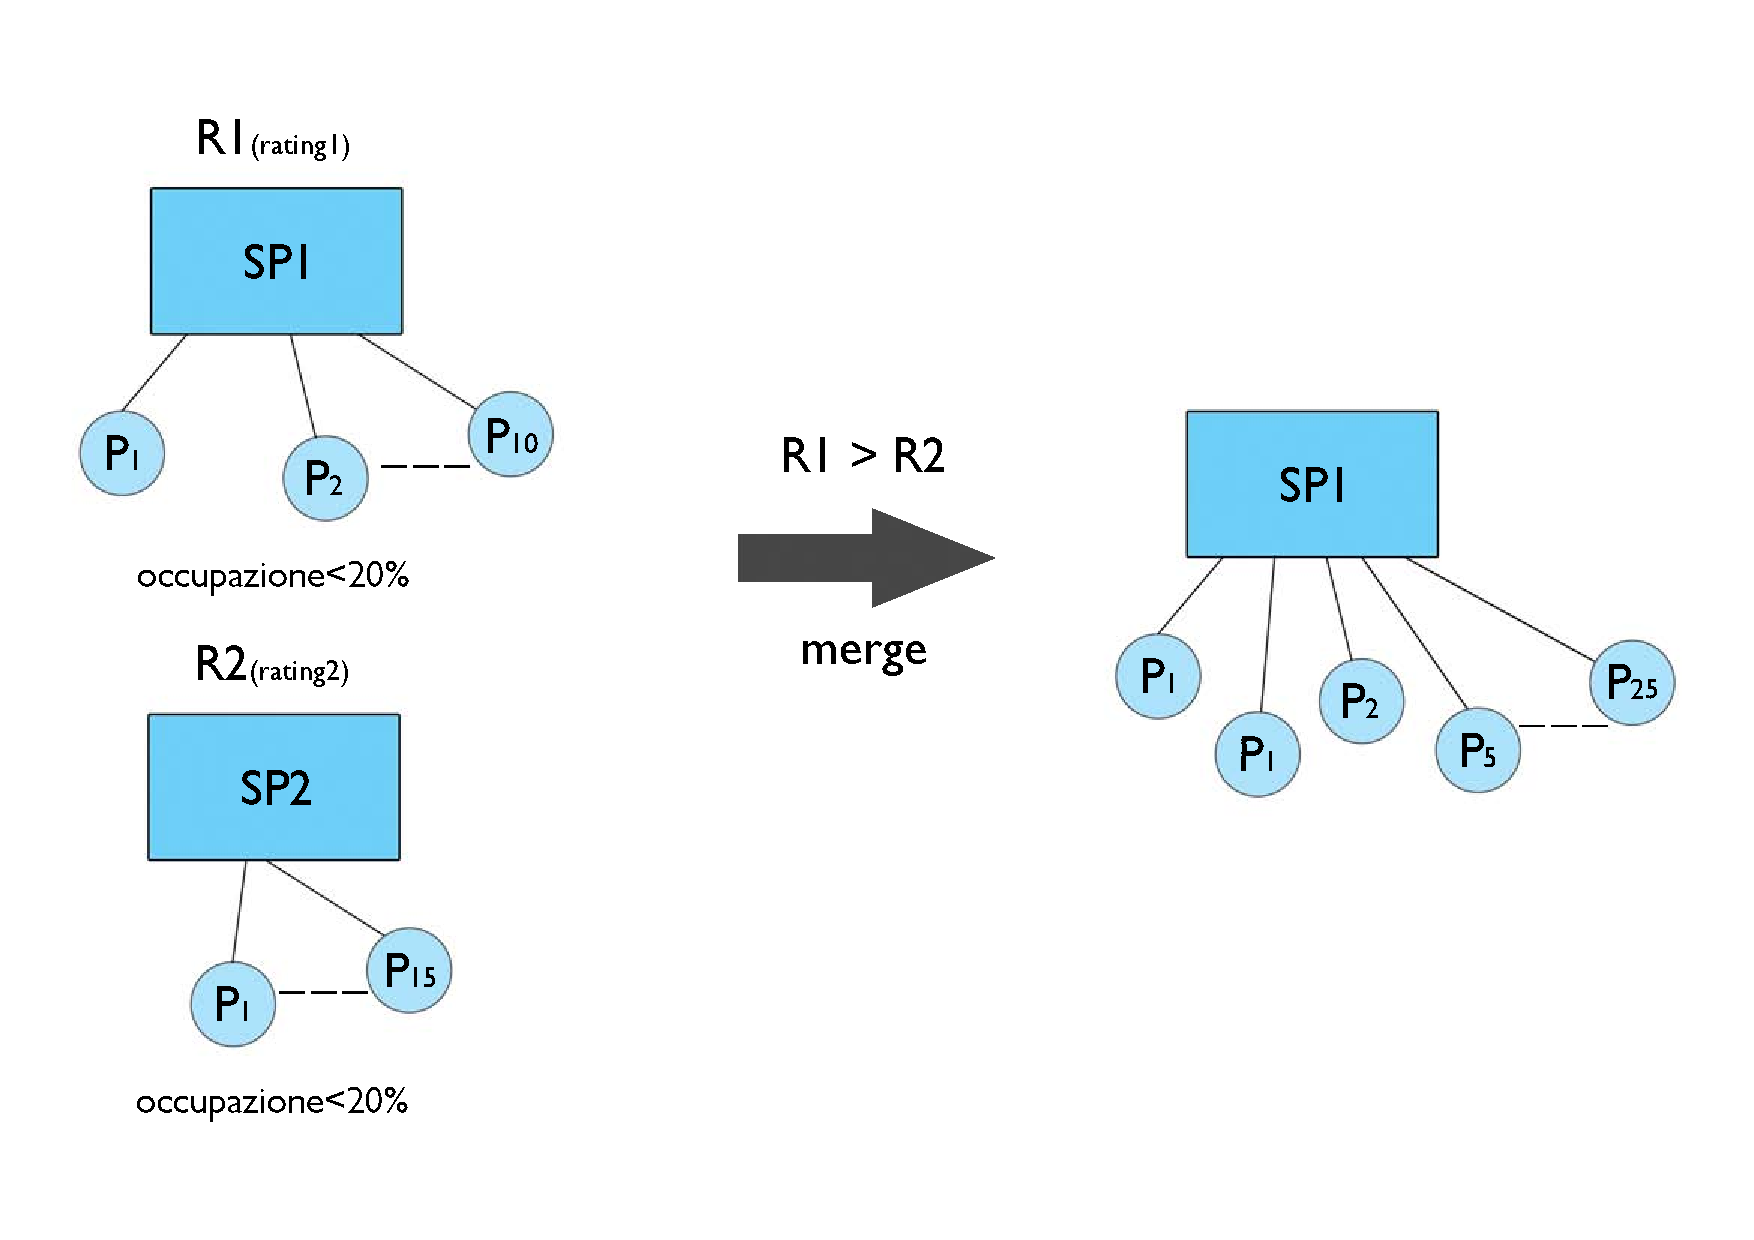
\includegraphics[width=10cm]{img/merge}}
\caption{merge tra due superpeer\label{merge}}
\end{figure}

\pagebreak


